\subsection{بخش ب}
در این بخش به بررسی تفاوت قانون هدایت تناسبی حقیقی و هدایت تناسبی افزوده پرداخته شده است.
\begin{table}[H]
	\caption{ فاصله ازدست‌دهی برای ضریب‌های مختلف تناسبی در قانون هدایت تناسبی حقیقی }
	\centering
	\begin{tabular}{cc}
		\hline
		\lr{Miss Distance (m)} &  \lr{Guidance Law} \\
		\hline
		$0.0834\!\times\!10^{-8}$ & \lr{TPN}\\
		$0$ & \lr{APN}\\
		\hline
	\end{tabular}
\end{table}

\begin{table}[H]
	\caption{ تلاش کنترلی برای ضریب‌های مختلف تناسبی در قانون هدایت تناسبی حقیقی }
	\centering
	\begin{tabular}{cc}
		\hline
		\lr{Control Effort} &   \lr{Guidance Law}  \\
		\hline
		$19.6963$ & \lr{TPN}\\
		$44.6641$ & \lr{TPN} \\
		\hline
	\end{tabular}
\end{table}

\begin{figure}[H]
	\centering
	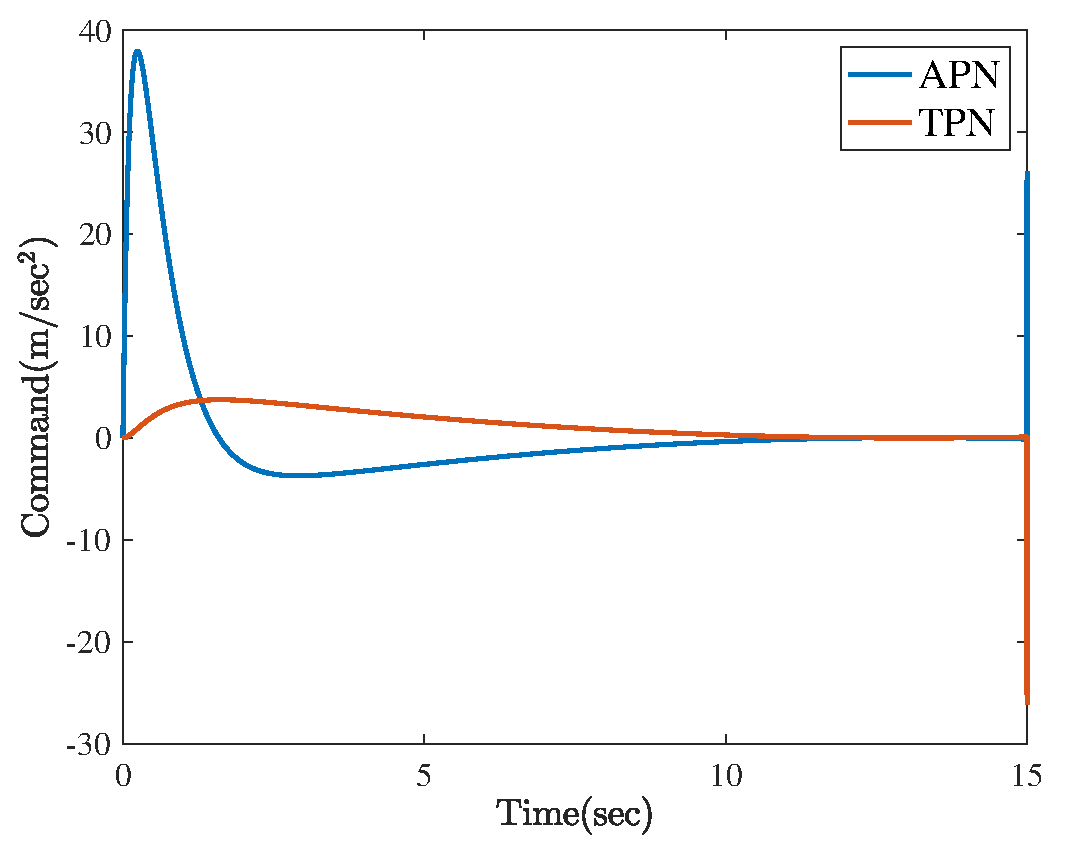
\includegraphics[width=.75\linewidth]{../Figure/Q2/b/command}
	\caption{مقایسه فرمان کنترلی در قانون هدایت تناسبی حقیقی و قانون هدایت تناسبی افزوده}
\end{figure}

\begin{figure}[H]
	\centering
	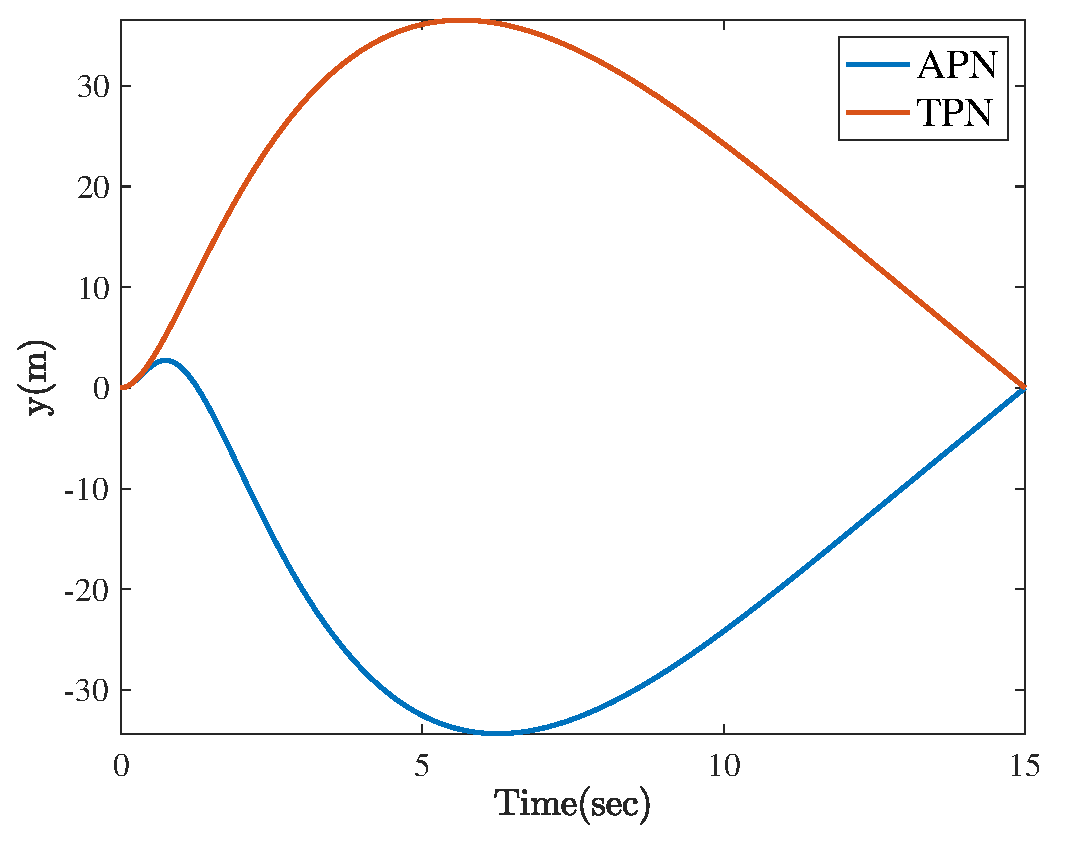
\includegraphics[width=.75\linewidth]{../Figure/Q2/b/y}
	\caption{مقایسه فرمان کنترلی در قانون هدایت تناسبی حقیقی و قانون هدایت تناسبی افزوده}
\end{figure}
